\documentclass[a4paper,8pt]{beamer}
\mode<presentation>
{
  \usetheme{Boadilla}
  % possiblities Singapore, Malmoe, Dresden 
  \setbeamercovered{transparent}
}

 
%\setbeamertemplate{navigation symbols}{} 
% removes the navigation symbols

%color setting more or less matching U of A colors
\setbeamercolor*{palette secondary}{use=structure,fg=white,bg=structure.fg!55!black}
\setbeamercolor*{palette tertiary}{use=structure,fg=white,bg=red!50!black}
%\usetheme{Madrid}
%\usecolortheme{seahorse}
\usepackage[retainorgcmds]{IEEEtrantools}
\usepackage{graphicx}
\usepackage{physics}
\usepackage{bm,bbm}
\usepackage{tabularx,multirow,booktabs}
\usepackage{subcaption}
\usefonttheme{serif}
\title[Free energy]{Research update}
\date{\today}
\author{Sree Ganesh}
\institute[U of A]{Schwartz Group \\ University of Arizona}
\begin{document}
\maketitle
%
%------------------------------------------------------------------------------
% SLIDE 6
%------------------------------------------------------------------------------
%
\begin{frame}
\frametitle{Window based sampling using the shooting algorithm}
    \begin{figure}[ht]
        \begin{minipage}[b]{0.45\linewidth}
            \centering
            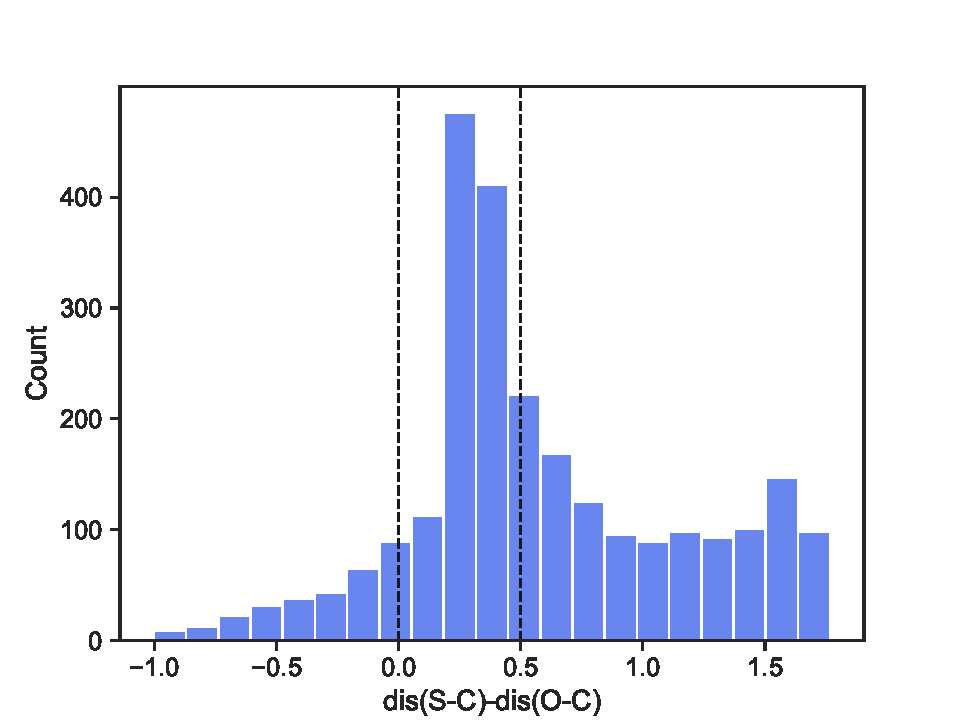
\includegraphics[width=\textwidth]{figures/window1.pdf}
            %\caption{Reac. traj. = 1, Non Reac. traj. =600}
            \label{fig:a}
        \end{minipage}
        \hspace{0.5cm}
        \begin{minipage}[b]{0.45\linewidth}
            \centering
            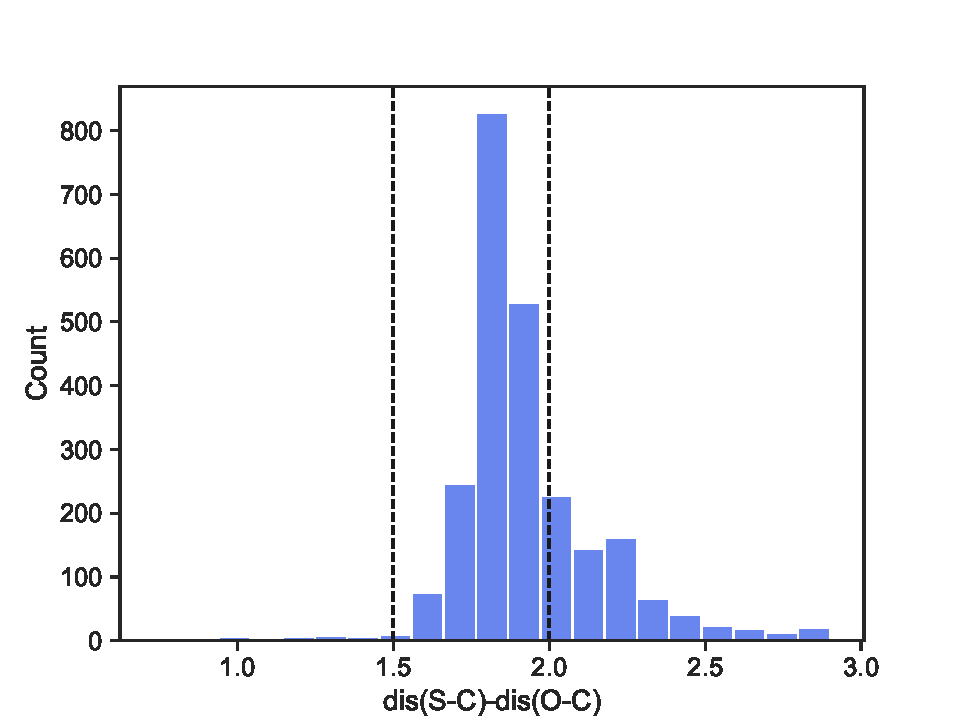
\includegraphics[width=\textwidth]{figures/window2.pdf}
            %\caption{Reac. traj. = 190, Non Reac. traj. =600}
            %\caption{QM region $+$ ARG 264, ARG 249, GLN 113 and SER 114 constrained.}
            \label{fig:b}
        \end{minipage}
    \end{figure}
\end{frame}
%
\begin{frame}
\frametitle{}
    \begin{figure}[ht]
        \begin{minipage}[b]{0.45\linewidth}
            \centering
            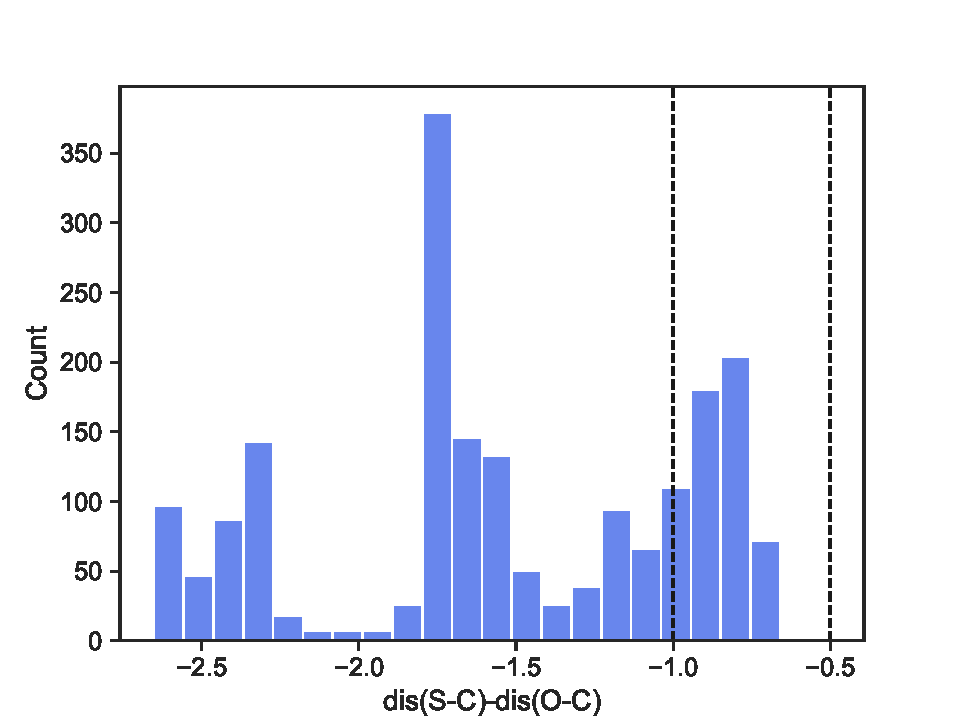
\includegraphics[width=\textwidth]{figures/window3.pdf}
            %\caption{QM region constrained.}
            \label{fig:a}
        \end{minipage}
        \hspace{0.5cm}
        \begin{minipage}[b]{0.45\linewidth}
            \centering
            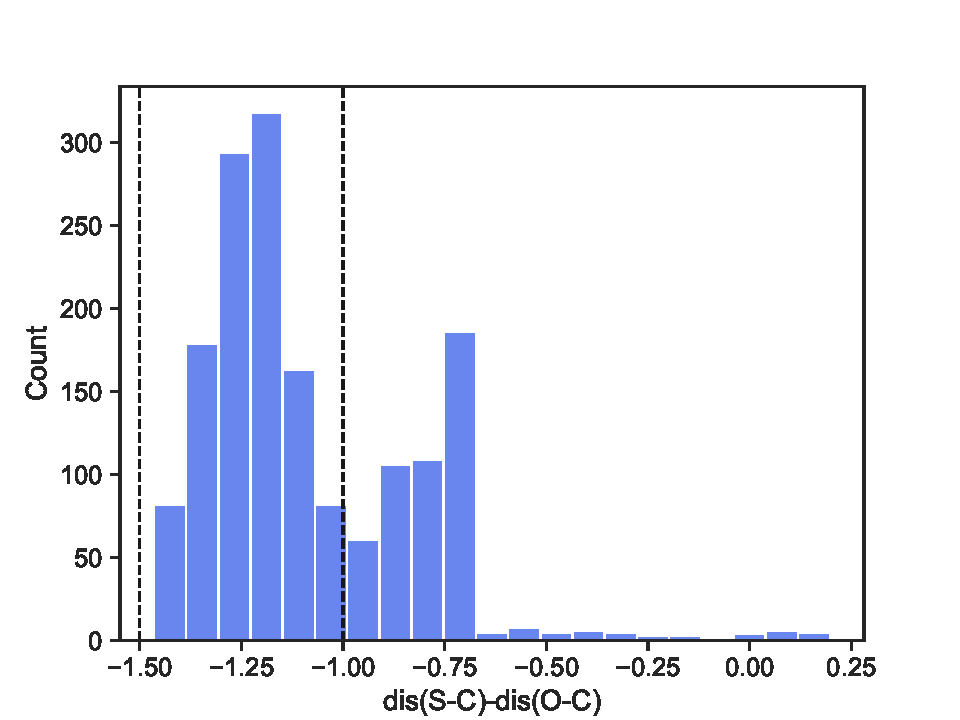
\includegraphics[width=\textwidth]{figures/window4.pdf}
            %\caption{QM region $+$ ARG 264, ARG 249, GLN 113 and SER 114 constrained.}
            \label{fig:b}
        \end{minipage}
    \end{figure}
\end{frame}
%
\begin{frame}
    \begin{figure}[ht]
        \begin{minipage}[b]{0.45\linewidth}
            \centering
            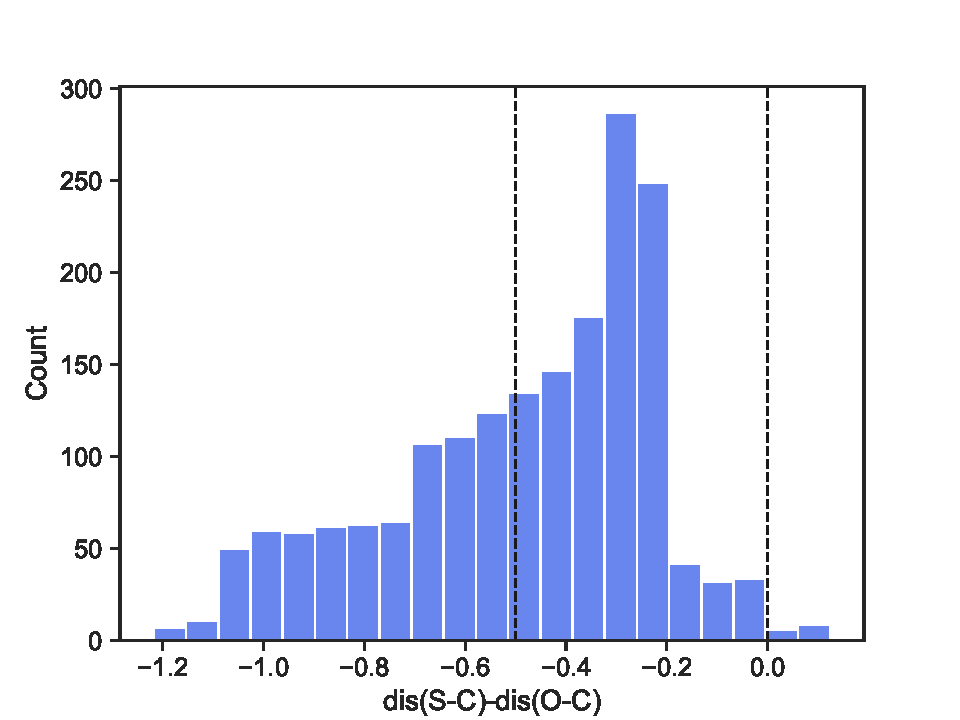
\includegraphics[width=\textwidth]{figures/window5.pdf}
            %\caption{QM region constrained.}
            \label{fig:a}
        \end{minipage}
        \hspace{0.5cm}
        \begin{minipage}[b]{0.45\linewidth}
            \centering
            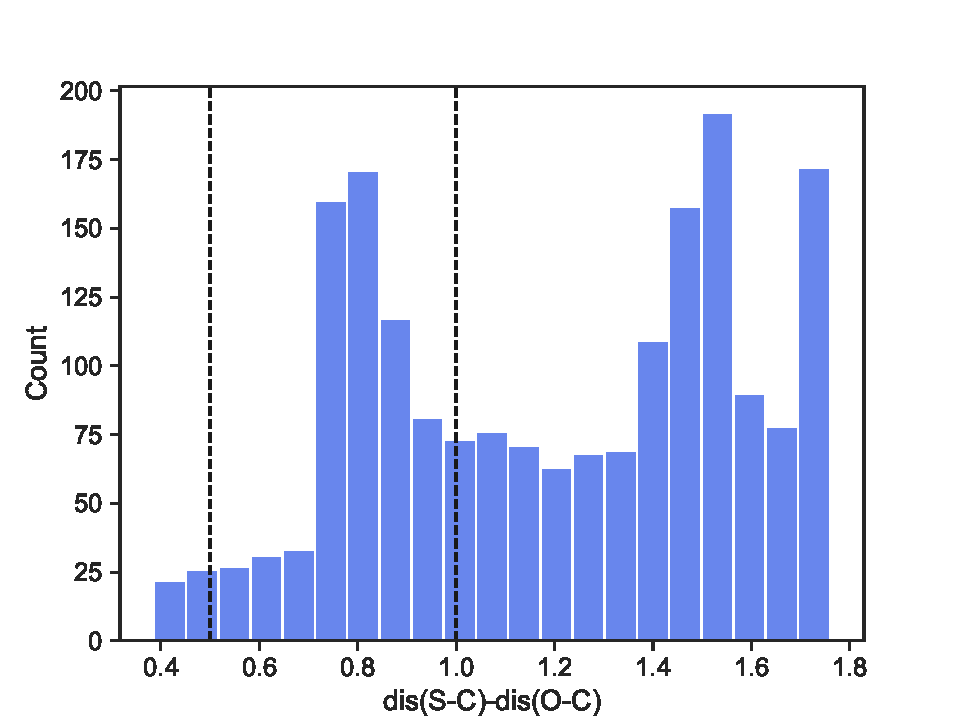
\includegraphics[width=\textwidth]{figures/window6.pdf}
            %\caption{Q}
            \label{fig:b}
        \end{minipage}
    \end{figure}
\end{frame}
%
\end{document}
